So far we have explored \textbf{Supervised Learning}, the goal of which is, given a set of data \((\textbf{X}, y)\), to learn a function that maps to \(\textbf{X} \longrightarrow y\). For example, regression or image captioning belong to this category of machine learning tasks.

Another fundamental class of tasks is \textbf{Unsupervised Learning}, which, given only the data \(\textbf{X}\), the algorithm learns some underlying hidden structure. For example, tasks such as clustering and density estimation belong to this class.

In general, models that belong to unsupervised learning can be divided into two categories: \textbf{non-probabilistic} and \textbf{probabilistic generative}. The latter will be the subject of this chapter. The goal of this class of models is to solve the so-called \textbf{density estimation} task.

Given a set of training data with a certain \texttt{distribution of training data} \(\sim p_{\text{\textbf{data}}}(x)\), the model aims to approximate this underlying distribution in order to generate new samples. To do this, the model learns a \texttt{distribution of generated samples} \(\sim p_{\text{\textbf{model}}}(x)\), such that \(p_{\text{\textbf{model}}}(x)\) is as close as possible to \(p_{\text{\textbf{data}}}(x)\).

We can further categorize the generative models according to whether the density of the samples has been explicitly specified or not, namely \textbf{Explicit Density Estimation Models} (e.g., \(p_{\text{\textbf{model}}}(x)\) should be a normal distribution whose parameters are unknown) and \textbf{Implicit Density Estimation Models}. An example of Explicit Density Estimation are VAEs, which explicitly define and solve for \(p_{\text{\textbf{model}}}(x)\). An example of Implicit Density Estimation are GANs, which learn a model that can sample from \(p_{\text{\textbf{model}}}(x)\) without explicitly defining it.

\section{Generative Adversarial Networks (GANs)}

The Generative Adversarial Networks, first introduced in the article \href{https://arxiv.org/pdf/1406.2661}{"Generative Adversarial Nets" (Goodfellow et al.)}, are probabilistic generative models that rely on implicit density functions. Instead, GANs exploit an \textbf{adversarial approach with two neural networks}: the \textbf{Generator} and the \textbf{Discriminator}.

The central role is that of the Generator: it learns to transform random noise into \textbf{complex samples that resemble those from a target distribution} (e.g., real images). This transformation process is supervised by the Discriminator, which simultaneously \textbf{learns to distinguish between real data samples and those generated by the Generator} (i.e., "fake" samples).

The adversarial aspect of this setup is crucial, where the Generator aims to produce samples indistinguishable from the real data in order to fool the Discriminator, while the latter tries to accurately differentiate between real and fake samples. This adversarial interaction drives both networks to improve iteratively, as each performance improvement in one network requires a corresponding adjustment in the other.

\newpage
\begin{figure}[!htbp]
    \centering
    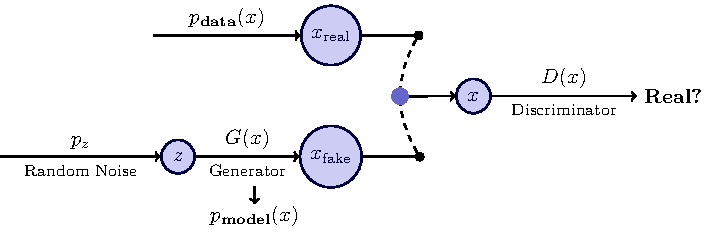
\includegraphics[width=\linewidth]{tikz/chapter9 - Generative Adversarial Network.pdf}
    \caption{GAN Architecture}
\end{figure}

As you can see, the Generator takes random noise \(z\) from a simple distribution \(p_z\) and transforms it into fake samples \( x_{\text{fake}} \) that resemble real data. The Discriminator receives both real samples \( x_{\text{real}} \) from the true data distribution \( p_{\text{\textbf{data}}}(x) \) and the fake samples from the Generator. It then classifies them as real or fake, \( D(x) \). The adversarial training process drives the Generator to produce increasingly realistic samples to fool the Discriminator, which in turn becomes better at distinguishing real from fake.

\subsection{Objective Function of GANs}

The training procedure involves two "players", the Generator and the Discriminator, who are jointly trained through a \textbf{min-max optimization problem}:

\vspace{-0.8cm}
{\Large

\begin{equation*}
min_{\theta_{g}} max_{\theta_{d}}\left[E_{x \sim p_{data}}  \log (\textcolor{mygreen}{D_{\tikzmarkk{Y}\theta_{d}}(x)}) + E_{z \sim p_{z}}\log (\textcolor{myred}{1-D_{\tikzmarkk{YC}\theta_{d}}(G_{\theta_{g}}(z))})  \right]
\end{equation*}
\begin{tikzpicture}[overlay,remember picture]
    \node (Ye) [below of = Y, node distance = 3.8 em, anchor=west] {\footnotesize \textsf{\textcolor{mygreen}{Discriminator Output for Real Data}}};
    \draw[<-, in=180, out=-90] (Y.south)++(.25em,-1ex) to (Ye.west);

    \node (YCe) [below of = YC, node distance = 2 em, anchor=west]     {\parbox{\widthof{Discriminator Output for}}{
    \ \\
    \footnotesize \textsf{\textcolor{myred}{Discriminator Output for}} \\ 
    \footnotesize \textsf{\textcolor{myred}{Generated Fake Data $G(z)$}}}};
    \draw[<-, in=180, out=-90] (YC.south)++(.25em,-.5ex) to (YCe.west);
\end{tikzpicture}
}

\vspace{1.4cm}
The Discriminator outputs a probability in the range (0,1) for real data. Each network has its parameters: \(\theta_{d}\) for the Discriminator and \(\theta_{g}\) for the Generator. Each module is described by a function, \(\mathbf{D_{\theta_{d}}(x)}\) and \(\mathbf{G_{\theta_{g}}(z)}\). 

The Discriminator (\(\theta_{d}\)) aims to maximize the objective such that \(D(x)\) is close to 1 (real) and \(D(G(z))\) is close to 0 (fake). Conversely, the Generator (\(\theta_{g}\)) aims to minimize the objective such that \(D(G(z))\) is close to 1 (tricking the Discriminator into believing \(G(z)\) is real).


\subsection{Training GANs}
During training, we use Stochastic Gradient Descent alternating between \textbf{gradient ascent} on the discriminator and \textbf{gradient descent} on the generator, respectively:

\vspace{-0.5cm}
{\Large
\begin{equation*}
\begin{aligned}
    &\max_{\theta_{d}} \left[E_{x \sim p_{data}} \log (D_{\theta_{d}}(x)) + E_{z \sim p_{z}} \log (1 - D_{\theta_{d}}(G_{\theta_{g}}(z))) \right] \\
    &\min_{\theta_{g}} \left[E_{z \sim p_{z}} \log (1 - D_{\theta_{d}}(G_{\theta_{g}}(z))) \right]
\end{aligned}
\end{equation*}
}

The function to be optimized is complex, so the training is \textbf{unstable}. In addition, it is very difficult to monitor the GAN process because the objective function is not related to the quality of the generated samples.

\begin{figure}[!htbp]
    \centering
    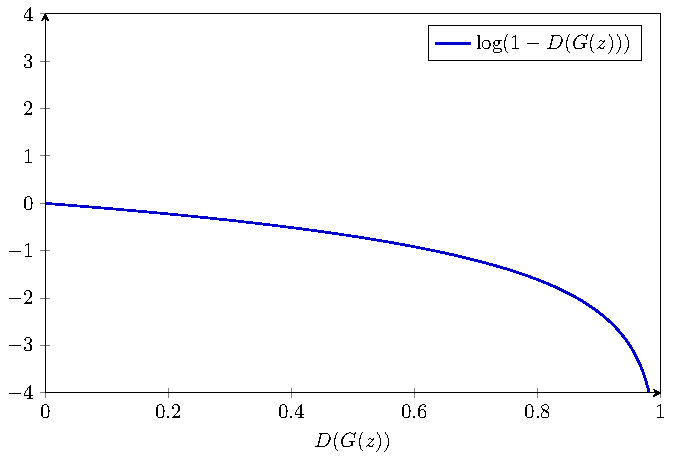
\includegraphics[width=0.7\linewidth]{tikz/chapter9 - SGD GAN Plot 1.pdf}
    \caption{SGD Plot for Generator during Training}
\end{figure}

In the figure, the line represents the gradient for the generator and the left part is when the generated sample is probably false. In this area, the gradient is quite \textbf{flat} and corresponds to the region where the model should learn more to improve its generating ability. In contrast, in the right part, the gradient signal dominates, which means that the sample is already good and not useful for learning purposes. Conceptually, \textbf{we waste a lot of resources in our area of interest, making learning more difficult}.

\begin{figure}[!htbp]
    \centering
    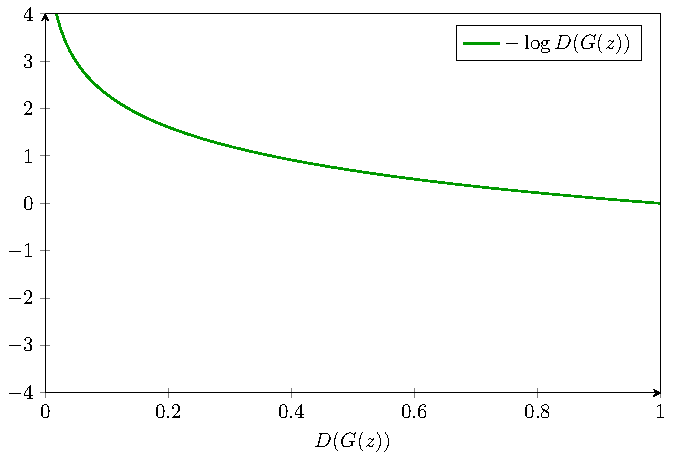
\includegraphics[width=0.7\linewidth]{tikz/chapter9 - SGD GAN Plot 2.pdf}
    \caption{SGD Plot (Inverted) for Generator during Training}
\end{figure}

Therefore, one way to improve training is to modify this part of the objective function and turn it into a \textbf{maximization problem}. This means that instead of minimizing the probability that the discriminator is correct, the model now \textbf{maximizes the probability that the discriminator is wrong}. As shown by the curve above, now the flat area has been inverted in the region outside our interest. Thus, the new training procedure requires alternating between two \textbf{ascending gradient} procedures:

\vspace{-0.5cm}
{\Large
\begin{equation*}
\begin{aligned}
    &\max_{\theta_{d}} \left[E_{x \sim p_{data}} \log (D_{\theta_{d}}(x)) + E_{z \sim p_{z}} \log (1 - D_{\theta_{d}}(G_{\theta_{g}}(z))) \right] \\
    &\ \textcolor{mybluee}{{\max_{\theta_{g}} \left[E_{z \sim p_{z}} \log (D_{\theta_{d}}(G_{\theta_{g}}(z))) \right]}}
\end{aligned}
\end{equation*}
}

Although the training efficiency has been improved, there are still some stability problems.

\subsection{Inference using GANs}
In probabilistic generative models, the inference phase is called the \textbf{sampling phase}: after training, the Discriminator is discarded and the Generator is used to produce samples similar to the training data from random noise.

Conceptually, the \textbf{Discriminator is just an auxiliary object} to match the distribution learned from the Generator with the distribution of our data.

The results showed that if this version of GAN is trained on an \textbf{unconstrained dataset}, i.e., one with a very wide distribution of labels (MNIST is a simple dataset since the digits have a similar distribution, while CIFAR-10 is a more complex one), it \textbf{performs poorly} regardless of the models used for both the Generator and the Discriminator (such as FC or CNN networks). However, the advantages of using the Generator network are that it can be used as a backbone for CNN or in NLP.

In the following sections, we will analyze the main problems of GANs and see some articles that have tried to mitigate them. These problems can be listed as follows:
\begin{itemize}
    \item \textbf{Overfitting and Control}: We do not have effective tools to determine whether the model is overfitting. The lack of clear indicators makes it difficult to implement techniques to control and prevent overfitting.
    \item \textbf{Evaluation of GANs}: There are no standardized and reliable metrics to evaluate the performance of a GAN. The quality of the samples generated can be subjective and difficult to quantify.
    \item \textbf{Training stability}: The training of GANs is notoriously unstable. 
    \item \textbf{Parameter oscillations and divergence}: Model parameters may oscillate or diverge during training. 
\end{itemize}

Another serious problem is the \textbf{Mode collapse}. This phenomenon occurs when the Generator, instead of capturing all modes of the target distribution, ends up capturing only one sub-mode, i.e., it learns only a certain area of the target distribution.

\begin{figure}[!htbp]
    \centering
    \includegraphics[width=0.8\linewidth]{tikz/chapter9 - Mode Collapse MNIST.pdf}
    \caption{Mode Collapse Example}
\end{figure}

The figure shows an example of mode collapse with the MNIST dataset: instead of learning to generate all the numbers, the Generator focuses only on one area of the overall distribution. As a result, after many iterations, it generates only number one.

Again, the figure below shows two rows of heatmaps representing the generator's distribution at different stages of training, from the initial phase (Step 0) up to 25K steps, along with the target distribution.

Both rows display the same sequence, but the crucial difference lies in how the model behaves in these two scenarios:

\begin{figure}[!htbp]
    \centering
    \includegraphics[width=\linewidth]{tikz/chapter9 - Mode Collapse HeatMap.pdf}
    \caption{Mode Collapse HeatMap}
\end{figure}

The top row illustrates the ideal behavior of the model, where the generator's distribution gradually converges towards the target distribution. In this case, we observe how the model successfully captures all data modes in a balanced manner.
    
The bottom row demonstrates the phenomenon of mode collapse. Here, despite the training steps being the same, we see that the model focuses on only one data mode at a time. At each step, the generator assigns a significant probability mass to a single mode, ignoring the others. This behavior persists throughout all training steps, and the model never achieves a distribution similar to the target.

This visual representation effectively highlights the problem of mode collapse: while the desired behavior is to model all data modes in a balanced way (as shown in the top row), in the case of mode collapse (bottom row), the model fixates on a single mode at a time, failing to capture the diversity of the target distribution.

\section{DCGANs}

Through the work of \href{https://arxiv.org/pdf/1511.06434}{"Unsupervised Representation Learning with Deep Convolutional Generative Adversarial Networks" (Radford et al.)}, the DCGAN model was introduced. This represents the first GAN architecture based on deep convolutional networks and was the first model to generate high-resolution images using GAN. In fact, multiple convolutional layers are used to produce high-quality images (64x64).

The architecture of the discriminator differs slightly from a classical CNN in that it \textbf{does not use pooling}, but only convolutions with stride. In principle, pooling is effective in models such as AlexNet because it helps avoid overfitting, but in GANs it negatively affects the discriminator's ability to judge whether an image is real or fake, making discrimination too easy.

In addition, Leaky ReLU is used as the activation function, and only one fully connected layer is present before the softmax output. For normalization, the model employs batch normalization after most levels.

Batch normalization is beneficial because it speeds up training, however, applied to DCGAN could lead to reduced performance because it \textbf{introduces correlation between samples within the minibatch}. The effect of correlation leads to a \textbf{loss of the diversity property} (samples not different enough) during the generation of samples by the Generator. As a result, the model will not be able to generalize.

\subsection{Arithmetic of GAN}

In the same paper, the authors explored the latent space of GANs trained on a dataset of celebrity faces. 

They found that, through training, \textbf{the generator learns to map points in the latent space} (which by itself has no intrinsic meaning) \textbf{to specific images}, and this mapping will be different each time the model is trained.

Also, the article showed that, to compute the output image, the generator performs \textbf{vector arithmetic with faces}. For example, the figure below shows that a smiling woman's face minus a neutral woman's face plus a neutral man's face results in a smiling man's face.

\begin{figure}[!htbp]
    \centering
    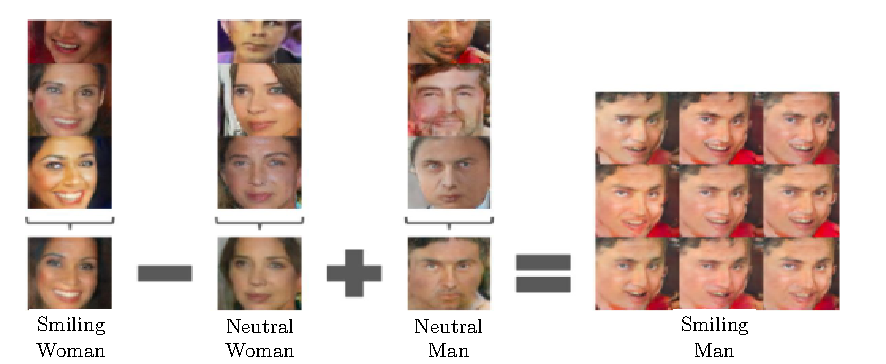
\includegraphics[width=0.8\linewidth]{tikz/chapter9 - Arithmetics of GAN.pdf}
    \caption{Example of Vector Arithmetic in GANs.}
\end{figure}

In this case, arithmetic is performed on the points in latent space corresponding to each resulting face. The results showed that the Generator has some interpolation capabilities (interpolation means that the vectors in latent space can be combined to obtain a sample whose features are a combination of the two).

\section{Evaluation of GANs}

Evaluating a GAN model is complex because of the lack of clear methods for assessing the visual quality of the generated images. The first attempt was the use of human feedback, which naturally involves problems of subjectivity and monetary costs.

Moreover, \textbf{we are not only interested in the quality of the generated images, but also in the overall distribution of the GAN-generated samples}, which should be similar to our dataset. However, there is no direct way to calculate the probability of high-dimensional samples (real or generated) or to compare their distributions.

Thanks to \href{https://arxiv.org/pdf/1511.01844}{"A note on the evaluation of generative models" (Theis et al.)}, we will explore two widely used metrics: \textbf{Inception Score} and \textbf{Fréchet Inception Distance (FID)}.

To simplify the evaluation problem, we can divide into two main properties: the ability of the GAN to generate \textbf{recognizable objects} and the \textbf{variety of objects} generated.
\begin{itemize}
    \item If the GAN produces concentrated distributions when it generates images belonging to the same class, it means that each of these images is associated with a high probability (\textbf{recognizable objects}) of belonging to that certain class.
    \item Globally, the dataset generated by GAN should be able to produce a \textbf{variety of objects}.
\end{itemize}

Both properties are associated with probability (likelihood). This is computed using a classifier, such as Inception-v3 (state of the art at the time). Then, we use its output (probability distribution) to calculate the inception score.

\begin{remark}{mygreen}{mygreen!15}
The inception score is calculated based on the output of an image classification model and is maximized if the entropy of the distribution of labels for the generated images is minimized (\textbf{recognizable}) and the predictions of the classification model are uniformly distributed over all possible labels (\textbf{variety}).
\end{remark}

However, this metric has an overfitting problem: with this method, a GAN that simply stores training data could still score well. If this statement does not make sense to you, try thinking, "\textit{Why would a GAN that generates samples that are very similar to my training set be useful?}" Obviously, such a model is not useful since it simply copies the images seen. 

Therefore, a better approach is to use the Fréchet Inception Distance (FID).

\begin{remark}{mybluee}{mybluee!15}
Using FID, both the real and the generated samples are passed through a classification network and for a chosen layer the activations are calculated. The metric then takes the embeddings of that layer and treats them as \textbf{multivariate normal distributions}. The mean and covariance are calculated for both the generated samples and the actual data and compared using Multivariate Normal Fréchet Distance. However, \textbf{the overfitting problem is not completely avoided}.
\end{remark}

\section{Different GAN Losses}

The loss function plays a key role in GANs: \textbf{different losses correspond to different ways of comparing the two distributions}.

Let us now analyze two different loss functions compared with the standard GAN: \textbf{LSGAN} and \textbf{Wasserstein GAN}.

LSGAN was introduced in \href{https://arxiv.org/pdf/1611.04076}{"Least Squares Generative Adversarial Networks" (Mao et al.)} with the goal of stabilizing the training of a GAN.

Cross entropy is replaced by \textbf{Least Square Loss}:

\vspace{-0.5cm}
{\Large
\begin{equation*}
\begin{aligned}
    &\min_{\theta_{d}} \left[\frac{1}{2}E_{x \sim p_{data}} \left(D_{\theta_{d}}(x) - 1\right)^2 + \frac{1}{2}E_{z \sim p_{z}} \left(D_{\theta_{d}}(G_{\theta_{g}}(z))\right)^2\right] \\
    &\min_{\theta_{g}} \left[\frac{1}{2}E_{z \sim p_{z}} \left(D_{\theta_{d}}(G_{\theta_{g}}(z)) - 1\right)^2\right]
\end{aligned}
\end{equation*}
}

This leads to better quality generated images (better IS and FID) and more robust generators to mode collapse:

\begin{figure}[!htbp]
    \centering
    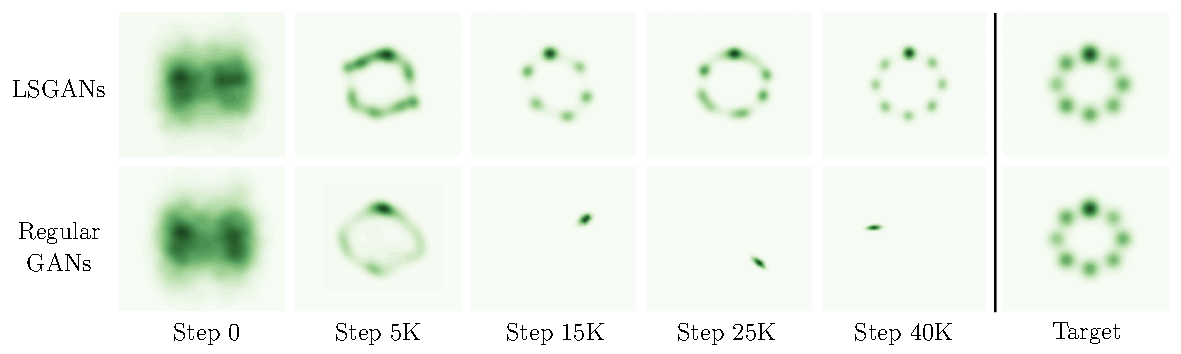
\includegraphics[width=\linewidth]{tikz/chapter9 - LSGAN.pdf}
    \caption{Results Comparison between LSGAN and Regular GAN}
\end{figure}

On the other hand, the work \href{https://arxiv.org/pdf/1701.07875}{"Wasserstein GAN" (Arjovsky et al.)} introduced the Wasserstein GAN with the idea of modifying the loss using a new method to better align the distributions of the dataset and the generated samples.

First, the \textbf{Wasserstein distance} is a metric that aligns two distributions with the concept of \textbf{optimal transport}. It measures the minimum cost of mass transport to convert the data distribution $q$ into the data distribution $p$.

Wasserstein GAN implements the idea of aligning the two distributions with this distance, providing \textbf{better gradients and more stable training}.

The most important result was that by implementing the Wasserstein GAN with the DCGAN architecture, it is possible to \textbf{correlate sample quality with the value of the Wasserstein distance}. This represents a huge improvement over other GANs. For example, not even DCGAN with the original divergence was able to achieve this property.

However, the more complex the distance, the more difficult the training becomes.

\newpage
\section{GANs Training Tricks}

In this section, we explore the tricks suggested in this paper: \href{https://arxiv.org/pdf/1606.03498}{"Improved Techniques for Training GANs" (Goodfellow et al.)}.


\begin{outline}
\textbf{Feature Matching} aims to stabilize GAN training by modifying the generator's objective. Instead of trying to directly deceive the discriminator, the generator focuses on \textbf{matching the statistics of features} from an intermediate layer of the discriminator. By minimizing the difference between these feature statistics for real and generated data, the generator avoids overfitting to the discriminator's current decision boundary, resulting in more stable training and higher-quality samples.
\\

\textbf{Mini-batch Discrimination} helps the generator produce more diverse outputs by allowing the discriminator to \textbf{examine relationships between samples in a mini-batch}. An additional layer in the discriminator computes differences between pairs of samples, providing information on how each sample compares to others in the batch. This enables the discriminator to identify if the generator is creating similar or identical samples, thus encouraging the generator to generate a wider variety of outputs and avoiding the problem of mode collapse.
\\

The \textbf{Virtual Batch Normalization (VBN)} is a normalization method that extends traditional batch normalization. Regular batch normalization makes the output of a neural network for an input example highly dependent on other inputs in the same minibatch. To avoid this problem, in VBN each example is \textbf{normalized based on statistics collected on a reference batch of examples} chosen once and fixed at the beginning of training, and on itself. The reference batch is normalized using only its own statistics. 
\end{outline}


\section{GANs Zoo}
Since their advent in 2014, GANs have gone through numerous iterations and improvements. In this section, we will embark on a journey through the "GAN Zoo", exploring how an initially simple concept has evolved into a multitude of innovative variations. 

\subsection{Conditional GAN}

Introduced in \href{https://arxiv.org/pdf/1411.1784}{"Conditional Generative Adversarial Nets" (Mirza et al.)},a Conditional GAN (cGAN) \textbf{links an input with its corresponding label}, enabling the use of supervised information. For example, a photo of a lion paired with the label "\textit{lion}" can be used to guide the generation process. \textbf{The optimization problem remains unchanged}, so the techniques and knowledge applied to standard GANs are still relevant.

In the cGAN framework, the generator incorporates the \textbf{label as an extension of the latent space}. This can be achieved by appending a one-hot encoded label vector to the latent spacez. The discriminator also utilizes the label information of real data, enhancing its ability to differentiate between real and generated samples. With this additional information, the discriminator can focus on a specific class, improving its performance.

\begin{figure}[!htbp]
    \centering
    \includegraphics[width=\linewidth]{tikz/chapter9 - Conditional GAN.pdf}
    \caption{Conditional GAN Architecture}
\end{figure}


\subsection{Image-to-Image Translation}

The paper \href{https://arxiv.org/pdf/1611.07004}{"Image-to-Image Translation with Conditional Adversarial Networks" (Zhu et al.)} introduces a conditional GAN architecture for image-to-image translation, known as \textbf{PIX2PIX Network}. The generative network transforms an input image into an output image, while the discriminative network evaluates how realistic and consistent the generated image looks with the input image. This approach is applicable to various tasks, such as translating photos into sketches, coloring black-and-white images, and improving image resolution. It is important to note that \textbf{training this model requires coupled/paired data}.


\subsection{Text-to-Image Synthesis}

Another interesting article is \href{https://arxiv.org/pdf/1605.05396}{"Generative Adversarial Text to Image Synthesis" (Reed et al.)}, which explores the use of GANs for image synthesis from textual descriptions. The generative network receives as input a textual description and a noise vector, and produces an \textbf{image that attempts to respect the content described in the text}. The discriminative network, on the other hand, distinguishes between real images with matching descriptions and generated images. This approach finds application, for example, in generating verbally described scenes or creating artwork from descriptions.

\subsection{Cycle GAN}



In the study \href{https://arxiv.org/pdf/1703.10593}{"Unpaired Image-to-Image Translation using Cycle-Consistent Adversarial Networks" (Zhu et al.)} an innovative methodology is introduced for translating images between two different domains, \textbf{overcoming the need for matching pairs of images}. For example, it is possible to transform photographic images into artworks in the style of Monet using CycleGAN, even when the two collections are not paired.

The CycleGAN model is based on \textbf{three main components}: the Discriminator, Generator and Translator networks, as follows:

\begin{itemize}
\item \textbf{Translator}: this network is responsible for "converting" an image from one domain (e.g., photographic images) to another domain (such as Monet paintings).

\item \textbf{Discriminator}: trained to determine whether an image belongs to the target domain. It also verifies that the translated image, when converted back to the original domain, actually looks similar to the source image.

\item \textbf{Generator}: this network takes care of transforming the translated image back to the original domain, trying to preserve fidelity to the initial version.
\end{itemize}


The CycleGAN architecture modifies the classical GAN training process by adding a \textbf{Cycle-Consistency Loss (similar to L1 loss)} to ensure that the image returned after translation and reconstruction is as close as possible to the original image.

\textbf{The model operates in both directions}: it translates an image from one domain to another and then brings it back. This operation is replicated by reversing the roles of the domains and sharing parameters between the two directions.

\begin{figure}[!htbp]
    \centering
    \includegraphics[width=0.4\linewidth]{tikz/chapter9 - CycleGAN Rolled.pdf}
    \caption{Cycle GAN Rolled Architecture}
\end{figure}

The figure represents the architecture of CycleGAN. On the top, the generative networks 
$G$ and $F$ handle the translation of images between the $X$ and $Y$ domains. The discriminators $D_X$ and $D_Y$ evaluate the generated images to confirm whether they belong to the respective domains. 

Below we have the "unrolled" versions of the model and the concept of Cycle-Consistency Loss is illustrated, which ensures that an image translated between the two domains and then reconverted retains a similarity to the original image.

\begin{figure}[!htbp]
    \centering
    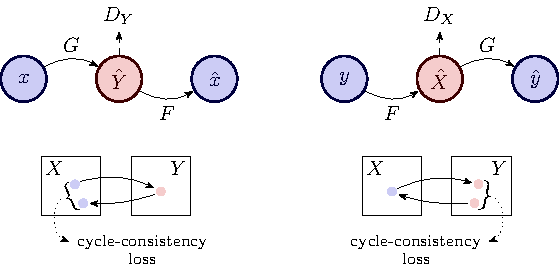
\includegraphics[width=\linewidth]{tikz/chapter9 - CycleGAN Unrolled.pdf}
    \caption{Cycle GAN Unrolled Architecture}
\end{figure}


\subsection{Progressive GAN}

\href{https://arxiv.org/pdf/1710.10196}{"Progressive Growing of GANs for Improved Quality, Stability, and Variation" (Laine et al.)} introduces the Progressive GAN model, which introduces a novel approach for generating high-quality images by a process of \textbf{progressive growth of the Generator and Discriminator networks}. This method involves the gradual expansion of the networks during training, thus enabling high-quality images.

\begin{figure}[!htbp]
    \centering
    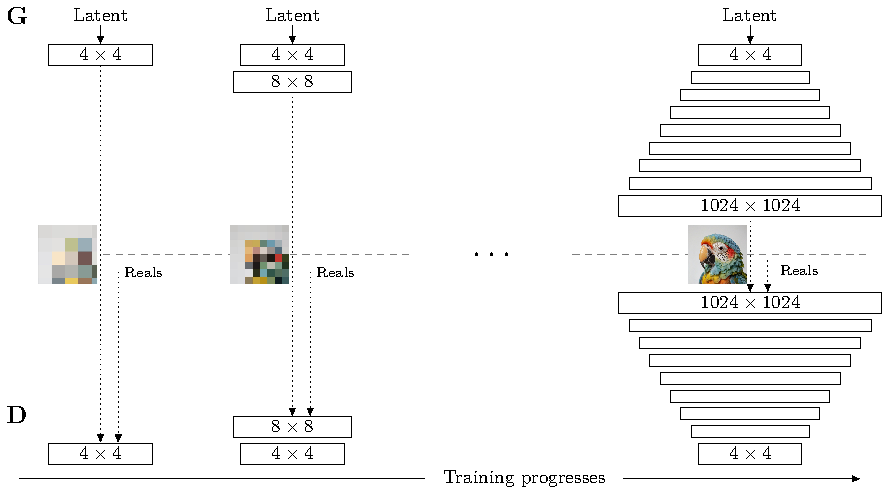
\includegraphics[width=0.9\linewidth]{tikz/chapter9 - Progressive GAN.pdf}
    \caption{Progressive GAN architecture}
\end{figure}

The principle behind this approach is that, at each stage of training, both networks benefit from the parameters learned in the previous stages. Initially, the networks work with smaller image sizes. As the training continues and stabilizes, new blocks of layers capable of handling larger images are added. This gradual growth process allows the model to \textbf{first learn the main structures and then refine the details}, thus improving the final quality of the generated images.


\subsection{Style GAN}

The model created by NVIDIA and described in the paper \href{https://arxiv.org/pdf/1812.04948}{"A Style-Based Generator Architecture for Generative Adversarial Networks" (Laine et al.)} is named StyleGAN and brings significant innovations to the architecture of GANs through the use of a Generator that is able to capture and manipulate in detail the \textbf{style attributes of images}, such as pose, hair type, or smile shape. It also allows these attributes to be modified stochastically, using random noise to vary the styles.

In the StyleGAN model, fundamental changes were made to the Generator architecture, such as the introduction of a \textbf{style vector}. This vector, derived from a latent representation via 8 fully connected layers (FC), captures the stylistic features of the image.

StyleGAN uses \textbf{Instance Normalization} to manage the stylistic attributes of images. This process calculates, for each image, the mean (\(\mu\)) and standard deviation (\(\sigma\)) of the pixel values. Normalizing the image with these statistics \textbf{removes the variations in brightness and color that are specific to each image, without altering the structure of the content.} The statistics \(\mu\) and \(\sigma\) then capture stylistic aspects such as texture and color. Instance Normalization is applied at different layers of the network to extract and control various aspects of style. These stylistic attributes are then reintegrated at the final generation stage, allowing precise control over the stylistic details of the final image.

\subsection{Drag GAN (2023)}

\textit{GANs are back with an exciting new feature!} \emoji{yum} DragGAN represents a recent advancement in GAN models, allowing interactive editing of images via a simple drag-and-drop method, as described in \href{https://vcai.mpi-inf.mpg.de/projects/DragGAN/}{"Drag Your GAN: Interactive Point-based Manipulation on the Generative Image Manifold" (Pan et al.)}.

In the DragGAN model, the user defines pairs of \textbf{control points} and \textbf{target points}, which indicate the areas of the image to be modified. The goal is to drag portions of the image from the position of the control points to the target points.

The optimization process is divided into two main steps:
\begin{enumerate}
    \item \textbf{Motion Supervision}: A module that guides the control points to the desired target points.
    \item \textbf{Point Tracking}: A module that continuously updates the position of control points to reflect changes.
\end{enumerate}

DragGAN demonstrates that, despite the emergence of more advanced models, GANs continue to innovate, offering practical and interactive solutions for image generation.


\section{Autoencoders}

Autoencoders are unsupervised models that learn to represent input data in a space of reduced size and then reconstruct it. This process occurs in two main steps: the encoder and the decoder.

\begin{figure}[!htbp]
    \centering
    \includegraphics[width=\linewidth]{tikz/chapter9 - Autoencoder.pdf}
    \caption{Autoencoder Architecture}
\end{figure}

The input is passed through the \textbf{Encoder}, a neural network that compiles data into a latent $z$ representation of lower dimension. This representation contains only the \textbf{most relevant features} extracted from the input. Next, the \textbf{Decoder}, which is a symmetric network with respect to the encoder, decodes the latent representation $z$ back to the size of the input to generate a reconstructed sample $x'$. The generated sample is then compared with the original input $x$ via a \textbf{reconstruction loss function (Norm L2)}.

The goal of training is to optimize the encoder and decoder weights to minimize this loss function. In particular, the encoder must refine its ability to extract essential features from the data, while the decoder must improve the quality of reconstruction of compressed features. After training, \textbf{the decoder part is generally discarded and the encoder can be used to initialize a supervised model} for predicting labels from the $z$ feature space.

Keeping the bottleneck ($z$) small forces the autoencoder to learn an intelligent representation of the data. Another approach to force the autoencoder to improve its representation is to add random noise to the inputs and have the model retrieve the original noise-free data, as described in the paper \href{https://www.cs.toronto.edu/~larocheh/publications/icml-2008-denoising-autoencoders.pdf}{"Extracting and Composing Robust Features with Denoising Autoencoders" (Bengio et al.)}, which introduces the \textbf{Denoising Autoencoders}.

In many modern autoencoder architectures, the encoder is implemented as a CNN, to compress the data into a more compact representation. The decoder, which has a similar but opposite structure to the encoder, uses \textbf{Transposed Convolution Layers} to reconstruct the original image from this compact representation. Transposed convolution layers work in the opposite way to the convolution layers used in the encoder: \textbf{while the encoder reduces the size of the image, the decoder increases it}. This is useful for recreating the image from the reduced representation.

\section{Variational Autoencoders (VAEs)}

Traditional autoencoders are designed to \textbf{replicate input data from the same dataset}. Variational autoencoders enhance this capability by learning distributions for latent features, allowing them to generate \textbf{unique images} with \textbf{similar features} to those in the training dataset. VAEs create a \textbf{continuous latent space} that facilitates sampling and interpolation, generating new samples that are similar to the inputs but different from those in the training set.

\begin{figure}[!htbp]
    \centering
    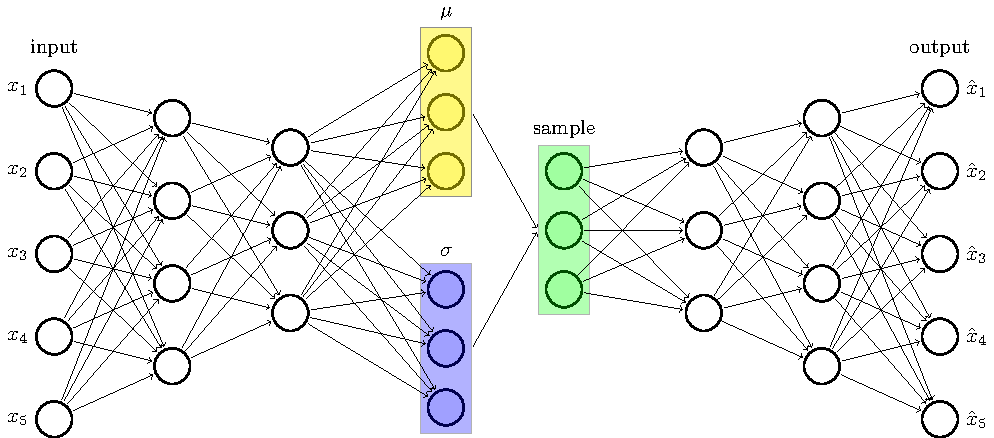
\includegraphics[width=\linewidth]{tikz/chapter9 - Variational Autoencoder.pdf}
    \caption{Variational Autoencoders Architecture}
\end{figure}

VAEs belong to the family of \textbf{explicit density estimation} models. Unlike models that indirectly measure the distribution of the data, VAEs use a direct approach to estimate the likelihood function of the data. The likelihood function for a sample of the dataset $x$ can be expressed as:

$$p_{\theta}(x)=\int_{} p_{\theta}(z)p_{\theta}(x|z)dz$$

where $z$ corresponds to the latent representation vector of our training data. 

The formula represents a likelihood function, thus we would like to learn the parameters $\theta$ that maximize it, i.e. such that generated data fit training data.

This formula represents a likelihood function, and the goal is to \textbf{learn the $\theta$ parameters that maximize it}, that is, those that best fit the generated data to the training data. However, we cannot compute this likelihood directly because it is mediated by $z$, which is a \textbf{latent representation learned from the training samples and not from the data itself}. Consequently, we do not have direct access to the data on which we are integrating.


To explain this problem, let us consider the formula in detail. It involves two probability distributions: $p_{\theta}(z)$ (\textbf{prior distribution}) represents the latent space, while $p_{\theta}(x|z)$ represents the Decoder, which samples $z$ from the prior distribution $p_{\theta}(z)$ and transforms it into a sample $x$ that must be similar to the training data.

Since the Decoder samples from the prior distribution, the latent space must be a simple probability distribution to facilitate this process. Therefore, the latent space is generally a \textbf{Gaussian Multivariate}. However, we cannot directly produce $p_{\theta}(z)$ since it is derived from the training data. \textbf{This is the integration problem}.

\textit{Here is a possible solution!} We could obtain $p_{\theta}(z)$ using Bayes' theorem. However, another problem would arise when we try to calculate the a posteriori probability distribution $p_{\theta}(z|x)$, since the denominator is intractable (\emoji{smiling-face-with-tear}):

$$p_{\theta}(z|x)= \frac{p_{\theta}(x|z)p_{\theta}(z)}{p_{\theta}(x)}$$

In this context, $p_{\theta}(z|x)$ represents the \textbf{latent space distribution extracted from the given input}.

\textbf{As usual in machine learning, the solution is VERY simple: we throw in a neural network.} In this case, the network is the \textbf{Encoder}, which is trained to map the input image to the latent space, $q_{\phi}(z|x)$. In this way, the encoder approximates the a posteriori distribution $p_{\theta}(z|x)$. \textbf{\textcolor{myred}{Beware that the encoder does not provide a global solution to the optimization problem, only an approximation: it provides a lower bound on the likelihood of the data!}}

Since we are modeling probabilistic data generation, both the encoder and the decoder are probabilistic models and are described by their own parameters, $\phi$ and $\theta$, respectively. The Encoder learns the mean and variance associated with the Gaussian distribution of the latent space $z$. The Decoder learns the mean and variance of the generating distribution, which should be as similar as possible to the dataset data.  \textbf{Then, the Variational Autoencoder can be seen as an Autoencoder with a probabilistic component}.

The objective function can be derived as follows by applying log-likelihood and several transformations:

\begin{equation*} 
\begin{aligned}
\log (p_{\theta}(x)) &= E_{z \sim q_{\phi}(z|x)}\left[ \log p_{\theta}(x) \right]\\
&=E_{z }\left[ \log \frac{p_{\theta}(x|z) p_{\theta}(z)}{p_{\theta}(z|x)} \right]  \text{  (Bayes Rule)} \\
&=E_{z }\left[ \log \frac{p_{\theta}(x|z) p_{\theta}(z)}{p_{\theta}(z|x)} \frac{q_{\phi}(z|x) }{q_{\phi}(z|x)}\right] \text{(Multiply by Constant)} \\
&=E_{z }\left[ \log p_{\theta}(x|z) \right] - E_{z} \left[ \log \frac{q_{\phi}(z|x)}{ p_{\theta}(z)}\right] + E_{z} \left[ \log \frac{q_{\phi}(z|x)}{p_{\theta}(z|x)} \right]  \text{(Logarithms)} \\
&=\textcolor{mybluee}{E_{z }\left[ \log p_{\theta}(x|z) \right] - D_{KL} \left[ q_{\phi}(z|x)|| p_{\theta}(z)\right]}\textcolor{mygreen}{\ + \ D_{KL} \left[ q_{\phi}(z|x)||p_{\theta}(z|x) \right]} 
\end{aligned}
\end{equation*}

From the equation above, \textbf{\textcolor{mygreen}{the third term is excluded}} since we cannot compute it, since we do not have access to $p_{\theta}(z|x)$ (remember, the encoder \textbf{approximates} the a posteriori distribution). However, this term is always a positive value since it is calculated via the KL divergence, which allows us to approximate the likelihood as a lower bound. If you do not know, \textbf{KL divergence is a measure of how similar two probability distributions are}; if they are identical, the divergence is zero, while a positive number indicates that the distributions are different.

\textbf{\textcolor{mybluee}{Two terms remain}}: the first is the Reconstruction Loss or \textbf{\textcolor{mybluee}{Reconstruction Term}}. This term is applied to the decoder to train it to \textbf{generate meaningful results} when it samples from the latent representation relative to the input data.

The second term can be computed in closed form because it involves the KL divergence between two Gaussian distributions and is used for the encoder (since it tries to approximate the prior distribution, which is a Gaussian). This is often called \textbf{\textcolor{mybluee}{Regularization Term}} because it \textbf{forces the latent space to fit a Gaussian distribution}.

\textbf{The combination of these two factors allows the latent space to be continuous and well-structured}, ensuring smooth interpolation between latent representations without gaps. This forces the encoder to produce a Gaussian distribution that approaches the prior.

\begin{figure}[!htbp]
    \begin{minipage}[t]{.3\textwidth}
        \centering
        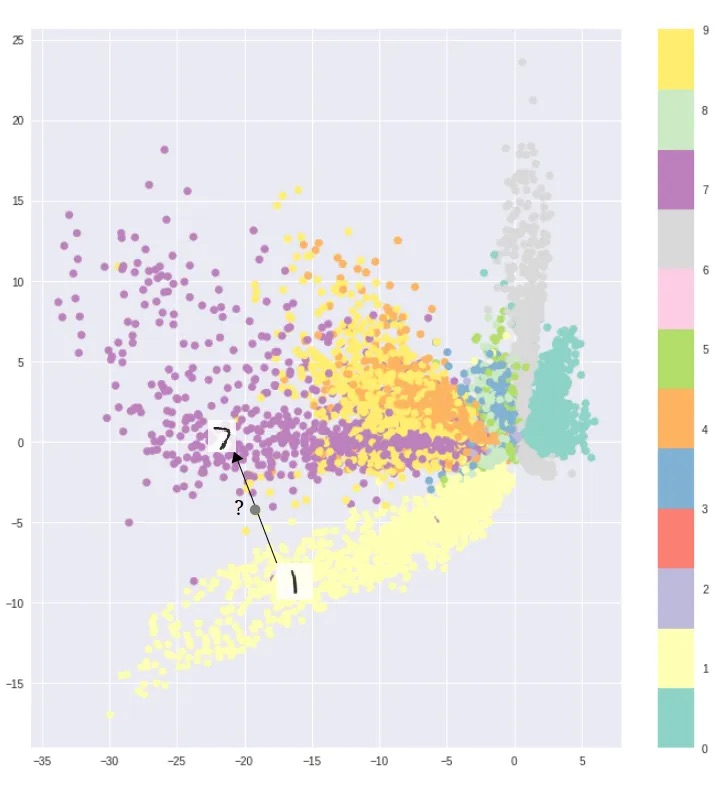
\includegraphics[width=\textwidth]{tikz/chapter9 - Latent Space VAEs 1.jpeg}
        \subcaption{Only Reconstruction Term}
    \end{minipage}
    \hfill
    \begin{minipage}[t]{.3\textwidth}
        \centering
        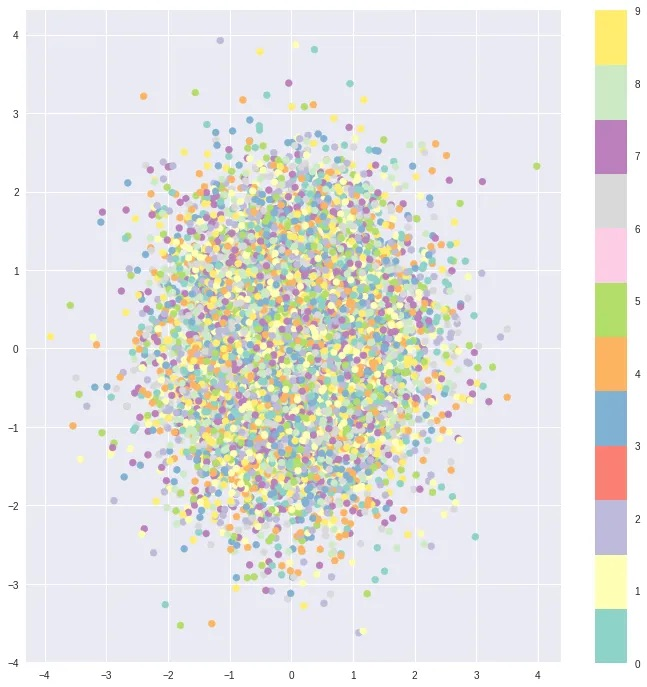
\includegraphics[width=\textwidth]{tikz/chapter9 - Latent Space VAEs 2.jpeg}
        \subcaption{Only Regularization Term}
    \end{minipage}  
    \hfill
    \begin{minipage}[t]{.3\textwidth}
        \centering
        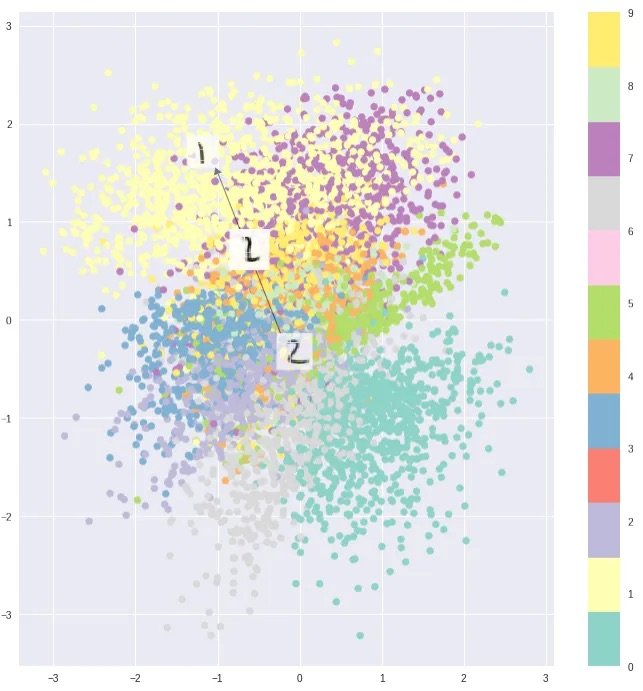
\includegraphics[width=\textwidth]{tikz/chapter9 - Latent Space VAEs 3.jpeg}
        \subcaption{Both}
    \end{minipage}  
    \caption{Latent Spaces Comparison}
\end{figure}

The figure compares three different latent spaces obtained by various autoencoder training strategies. 

The latent space on the left is the result of \textbf{exclusive use of reconstruction loss}, as in traditional autoencoders. In this case, no constraint is applied on the latent space distribution. As can be seen, the latent space has no well-defined structure and the latent points are not distributed according to a centered Gaussian. In other words, the latent data appear scattered and disorganized, with no clear structure. \textit{Indeed, autoencoders are not generative models by nature, since there are no constraints on the latent space to guarantee its structured behavior. If we train an autoencoder, take the latent space and add noise, the decoder will produce meaningless results. }

The second latent space, located in the center of the figure, is obtained by using \textbf{only the regularization term}. In this scenario, the model learns a narrower distribution for each sample type, trying to fit a Gaussian shape. However, as highlighted in the figure, although the distribution assumes a Gaussian shape, the latent points tend to overlap and mix. This makes it difficult to distinguish the different data sets, as the latent data are not well separated.

Finally, the latent space on the right represents the result of \textbf{joint optimization of both terms: the reconstruction loss and the regularization term}. This combination allows the latent space to fit the data well, being continuous and similar to a Gaussian distribution. As a result, the latent space presents a uniform and continuous structure, with the data distinct in well-defined clusters, exactly what we want to achieve! \emoji{smiling-face-with-sunglasses}


Now, \textbf{to train VAEs we want to use backpropagation, but in practice this is impossible} (\emoji{pensive}) because sampling from the latent distribution $z \sim q_{\phi}(z|x)$ is not differentiable. \textit{However, the \textit{\textbf{reparametrization trick}} comes to our rescue!} This trick is to sample from a standard normal distribution $\epsilon \sim \mathcal{N}(0, I)$ and transform it with $z = \mu(x) + \sigma(x) \cdot \epsilon$. So, \textbf{the sampling process becomes differentiable with respect to the model parameters}, facilitating the training of latent representations. \emoji{smiling-face-with-sunglasses} (again)


\section{VQ-VAEs}

Typically, in a classic VAE, the prior ($p_{\theta}(z)$) and posterior ($q_{\phi}(z|x)$) are assumed to be normally distributed with diagonal variance. In the proposed work on VQ-VAEs \href{https://arxiv.org/pdf/1711.00937}{"Neural Discrete Representation Learning" ( van den Oord et al.)}, however, the authors use \textbf{discrete latent variables} (instead of a continuous normal distribution). The posterior and prior distributions are categorical, and \textbf{samples drawn from these distributions index a embedding table}. Then, the encoders model a \textbf{categorical distribution}, from which we sample to obtain integral values. These integral values are used to index an embedding dictionary, and the indexed values are then passed to the decoder.

For example, in images we may have categories such as "Dog" or "Bicycle," and it would not make sense to mix these categories. Discrete representations are also easier to handle, since each category has a unique value. In contrast, in a continuous latent space, it would be necessary to normalize the density function and understand the relationships between the various variables, which can be very complicated.
    

\section{GAN and VAE Comparison}

\begin{table}[!htbp]
\centering
\begin{tabular}{|l|c|c|}
\hline
& \textbf{GANs} & \textbf{VAEs} \\
\hline
Efficient sampling & \cellcolor{mygreen!15}\checkmark & \cellcolor{mygreen!15}\checkmark \\
\hline
High quality & \cellcolor{mygreen!15}\checkmark & \cellcolor{myred!15}$\times$ \\
\hline
Coverage & \cellcolor{myred!15}$\times$ & \cellcolor{myblue!15}? \\
\hline
Well-behaved latent space & \cellcolor{mygreen!15}\checkmark & \cellcolor{mygreen!15}\checkmark \\
\hline
Interpretable latent space & \cellcolor{myblue!15}? & \cellcolor{myblue!15}? \\
\hline
Efficient likelihood & \cellcolor{myorange!15}n/a & \cellcolor{myred!15}$\times$ \\
\hline
\end{tabular}
\caption{GAN and VAE Comparison}
\end{table}

\textbf{Comparison of GAN and VAE using the Ideal Properties of Generative Models}

\textbf{High-Quality Sampling}: GANs are capable of generating high-quality samples, meaning the samples they produce are often indistinguishable from real data.

\textbf{Coverage}: GANs often struggle with coverage, meaning they might generate samples that represent only a subset of the training data, rather than covering the entire distribution. VAEs generally aim to cover the full distribution, though their success in this area can vary.

\textbf{Well-Behaved Latent Space}: Both models have well-behaved latent spaces. In other words, each latent variable $z$ corresponds to a realistic data example $x$, and smooth changes in $z$ lead to smooth changes in $x$.

\textbf{Interpretable Latent Space}: Neither GANs nor VAEs excel at providing an interpretable latent space. Ideally, altering each dimension of $z$ should affect a specific, understandable feature of the data, but neither model achieves this effectively.

\textbf{Efficient Likelihood Computation}: VAEs, despite being probabilistic models, struggle with efficiently computing likelihoods. GANs do not use likelihoods, so this characteristic does not apply to them.
